%%%%%%%%%%%%%%%%%%%%%%%%%%%%%%%%%%%%%%%%%%%%%%%%%%%%%%%%%%%%%%%%%%%%%%%%%%%%%%%%
% Introduction 已经完工 可小改
% 搜索 TODO 找没写的部分
%%%%%%%%%%%%%%%%%%%%%%%%%%%%%%%%%%%%%%%%%%%%%%%%%%%%%%%%%%%%%%%%%%%%%%%%%%%%%%%%

\chapter{Introduction}
\label{ch:intro}

  \section{Purpose}
  The purpose of this document is to build a command-line version of the game Monopoly. In the game, players roll dices to move around the game board triggering events, and win by economical domination. \par

  \section{Document Conventions}

    \subsection{Requirements}
      This document uses a indexing of form \texttt{[DEMO-REQ-1]} where preceding letters denote requirement category and the number denotes the index. For instance, \texttt{[GAME-RULE-2]} represent the second requirement in the \hyperref[sec:game-rules]{game rule} section. \par

    \subsection{Acronyms and Abbreviations}
      This document adopts the following abbreviation conventions. \par
      \begin{table}[!htbp]
        \centering
        \begin{tabular}{*2c}
          \toprule
          Abbreviation & Full Form \\
          \midrule
          ER & Entity Relationship \\
          ID & Identifier \\
          SRS & Software Requirement Specifications (Document) \\
          \bottomrule
        \end{tabular}
        \caption{Acronyms and Abbreviations}
        \label{table:abbr}
      \end{table}

  \section{Intended Audience and Reading Suggestions}
    This document is most useful for development team, project managers, supervisors and documentation writers. \par
    The rest of this document are organized according to the following: \par
    \begin{itemize}
      \item Chapter \textit{\hyperref[ch:intro]{Introduction}} provides basic information on this project and this document.
      \item Chapter \textit{\hyperref[ch:overall-desc]{Overall Description}} presents an overview of this project, describing its functions, users, environments and development in details.
      \item Chapter \textit{\hyperref[ch:sys-req]{System Requirements}} indicates all the functional and non-functional requirements in more detail.
      \item Chapter \textit{\hyperref[ch:apdx]{Appendices}} includes the most detailed yet trivial information related to this project or this document.
    \end{itemize}

  \section{Product Scope}
    This document specifies requirements for the command-line game Monopoly. \par
    This software allows users to: \par
    \begin{itemize}
      \item View the game board and players' token (subject to change in each round)
      \item Roll the in-game virtual dices to make a move
      \item Manage in-game assets (e.g. money, estates)
      \item Deal with in-game triggered events
      \item Save/load a game
    \end{itemize}
    The software runs offline without connection to any server, and stores game on local disk. The software displays game progress and interacts with users through command-line prompts and inputs respectively. 

  \section{References}
    \begin{itemize}
      \item COMP3211 Software Engineering Course Project Description
      \item \href{https://en.wikipedia.org/wiki/Monopoly_(game)}{Monopoly - Wikipedia}
      \item \href{https://www.overleaf.com/latex/templates/cse355-software-requirements-specification-layout/pvjpzxthtngc}{SRS Template}
      \item \href{https://www.reqview.com/papers/ReqView-Example_Software_Requirements_Specification_SRS_Document.pdf}{SRS Example}
    \end{itemize}

\chapter{Overall Description}
\label{ch:overall-desc}

  \section{Product Perspective}
    \begin{table}[!htbp]
      \centering
      \begin{tabular}{c|c}
        \toprule
        \multirow{3}{*}{OS} & Windows 7(64-Bit) or above;  \\
        & or MacOS OSX 10.12 or above; \\
        & or Major Linux Distribution from 2010 \\
        \midrule
        Processor & 1.5 GHZ or above \\
        \midrule
        Memory & 500 MB free memory or above \\
        \midrule
        Storage & 100 MB free space or above \\
        \midrule
        Software & JSE 8 or above or Python 3 \\
        \bottomrule
      \end{tabular}
      \caption{Operating Environment}
      \label{table:opr-env}
    \end{table}
    
    \subsection{System Interfaces}
      The application runs in the Python shell or JVM on Windows, Mac or Linux.

    \subsection{User Interfaces}
      The application offers a command line interface, displaying a game board. During interactions, the application prompts with available options, and accepts input from the user.

    \subsection{Software Interfaces}
      The application allows storing and loading a game as a file, in which game status is preserved, so that the game can be consistent after the store-and-load cycle.

    \subsection{Assumptions and Dependencies}
      \begin{itemize}
        \item JSE 8 or above or Python 3 has to be installed for the application to start
        \item System should use a proper font to support UTF character set to correctly diaplay the game board
      \end{itemize}

  \section{Product Functions}

    \subsection{User Requirements Definition}
      % SEE User Requirements Definition
      Users should be able to: \par
      \label{sec:user-needs}
      \begin{enumerate}[label=\texttt{[USER-NEEDS-\arabic*]}:, leftmargin=10em]
        \item Start or load a game from main menu.
        \item Quit (with or without saving) or restart in the middle of a game.
        \item Quit or restart after a game ends.
        \item During the game, observe the progress of the game.
        \item During the game, observe the location of all game tokens.
        \item During the game, control to roll the dices.
        \item During the game, decide for incoming options (e.g. owning a property, paying a fine, etc.).
      \end{enumerate}

    \subsection{Requirements Storage}
      Below table demonstrates the mapping between user need and its storage method accompanied with corresponding functions to support its role.
      \begin{table}[!htbp]
        \centering
        \begin{tabular}{c|c|c}
          \toprule
          User Need & Storage & Supporting Functions \\ 
          \midrule
          \multirow{4}{*}{\shortstack[l]{\texttt{[USER-NEED-1]} \\ \texttt{[USER-NEED-2]} \\ \texttt{[USER-NEED-3]}}} & \multirow{2}{*}{Game Saves} & saving a game in a file;  \\
          & & loading a game from a file. \\
          \cmidrule{2-3}
          & \multirow{2}{*}{AUTOSAVE} & instantly saves all the changes; \\
          & & restores the game when the system is restarted. \\
          \bottomrule
        \end{tabular}
        \caption{User Requirement Storage}
        \label{table:req-storage}
      \end{table}

  \section{User Classes and Characteristics}
    Users who know the basics of command line operations, such as opening a terminal, opening the game, following the instruction to type in-game commands.
    %一个应该差不多了 也没啥别人会玩
    %<Identify the various user classes that you anticipate will use this product. User classes may be differentiated based on frequency of use, subset of product functions used, technical expertise, security or privilege levels, educational level, or experience. Describe the pertinent characteristics of each user class. Certain requirements may pertain only to certain user classes. Distinguish the most important user classes for this product from those who are less important to satisfy.>

\chapter{System Requirements}
\label{ch:sys-req}

  \section{Functional Requirements}

    \subsection{Main Menu Operations}
      \begin{enumerate}[label=\texttt{[FUNC-REQ-\arabic*]}:, leftmargin=10em]
        \item The application should scan for local game saves. If none, prompt for users to start a new game, otherwise, prompt for users to choose between starting a new game and loading from game save.
        \item When starting a new game, the application shall prompt to ask the number of players in the game (ranged from 2 to 6).
      \end{enumerate}

    \subsection{Game Save Operations}
      \begin{enumerate}[label=\texttt{[FUNC-REQ-\arabic*]}:, start=2, leftmargin=10em]
        \item During a game, the application shall allow users to save a game to a local game save, with its name specified.
        \item The application shall automatically save the current progress during a game to a local game save with a fixed name "AUTOSAVE" (overwrite if conflict exists), which later can be loaded by the user, at a specific frequency.
        \item The application shall allow users to load a game, by displaying all available local game saves and then prompt for user's choice.
      \end{enumerate}

    \subsection{Game View}
      \begin{enumerate}[label=\texttt{[FUNC-REQ-\arabic*]}:, start=5, leftmargin=10em]
        \item The application shall display a game board, containing all player tokens and game status (current active player ID or name, their current balance, and current round number).
        \item The application shall automatically prompt for switch of player between turns. 
        \item The application shall prompt description of operation needed along with available options for users to take action. The description and options are subject to both  \hyperref[sec:game-rules]{game rules} and \hyperref[sec:board-specs]{game board specifications}.
        \item THe application shall prompt the result of the actions (e.g. present a change in user's  balance).
        \item The application shall support quit and restart options at any moment of the game.
      \end{enumerate}
      
    \subsection{System Architecture}
      \begin{itemize}
        \item Game: The main class, processing user input, main game logic, event systems and system actions such as start/end/save/load. 
        \item Printer: The printer class, printing game prompts and game board during the game.
        \item Player: holding basic information of players such as name, wealth, position and poccessions.
        \item Building: holding building information on each cell.
        \item Event: describing events
        \item Funcs: describing details of event operations
      \end{itemize}

      \begin{figure}[ht!]
        \centering
        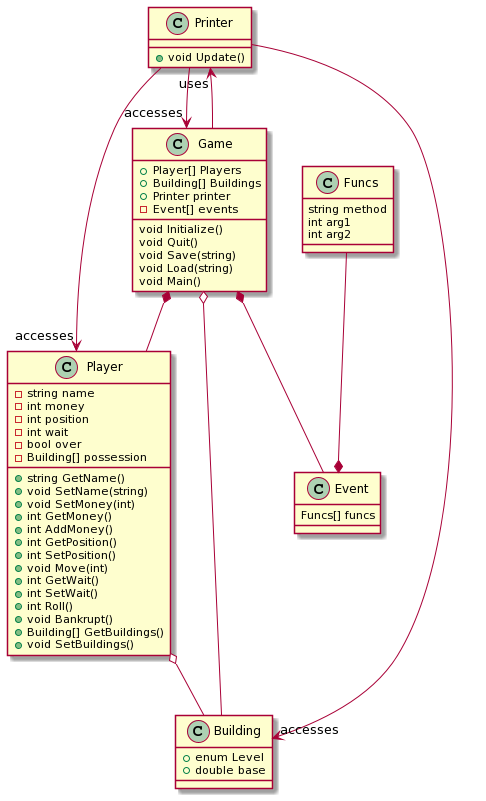
\includegraphics[width=0.8\textwidth]{image/UML.png}
        \caption{Class Diagram}
        \label{fig:class-diagram}
      \end{figure}
  
  \section{Non Functional Requirements}

    \subsection{Performance Requirements}
      \begin{enumerate}[label=\texttt{[NFUNC-REQ-\arabic*]}:, leftmargin=10em]
        \item The application should occupy at most 2 GB of system memory.
        \item The application should load a game save within 10 seconds.
        \item The application shall process and respond to user input within 1 second.
        \item The application shall limit its average game save size to 10MB.
        \item The application shall include simple animations when displaying dynamic content.
      \end{enumerate}

    \subsection{Software System Attributes}
      \begin{enumerate}[label=\texttt{[NFUNC-REQ-\arabic*]}:, leftmargin=10em]
        \item The application should not send any daat to the Internet.
        \item The application shall sanitize any data input or imported by users.
        \item The application can produce game saves in either encrypted or unencrypted form.
        \item The application shall forbid access over local storage other than its root directory or a specific location, in order to prevent malpractices on user data.
      \end{enumerate}

\chapter{Appendices}
\label{ch:apdx}

  % TODO 
  % \section{Index}
  \section{Game Design Specifications}
  \label{ch:game-design-specs}

    \subsection{Game Board Specifications}
    \label{sec:board-specs}
      \begin{figure}[ht!]
        \centering
        \includegraphics[width=0.8\textwidth]{image/image-000.jpg}
        \caption{Monopoly Game Board Schematic Diagram}
        \label{fig:game-board}
      \end{figure}
      \begin{table}[!htbp]
        \centering
        \begin{tabular}{c|c|c|c}
          \toprule
          Position Index & Name & Selling Price & Rental Price \\
          \midrule
          2 & Central & 800 & 90 \\
          3 & Wan Chai & 700 & 65 \\
          5 & Stanley & 600 & 60 \\
          7 & Shek O & 400 & 10 \\
          8 & Mong Kok & 500 & 40 \\
          10 & Tsing Yi & 400 & 15 \\
          12 & Shatin & 700 & 75 \\
          14 & Tuen Mun & 400 & 20 \\
          15 & Tai Po & 500 & 25 \\
          17 & Sai Kung & 400 & 10 \\
          18 & Yuen Long & 400 & 25 \\
          20 & Tai O & 600 & 25 \\
          \bottomrule
        \end{tabular}
        \caption{Selling and Rental Price of each Property}
        \label{table:property-price}
      \end{table}
      \begin{enumerate}[label=\texttt{[BOARD-SPECS-\arabic*]}:, leftmargin=10em]
        \item There are in total 20 circularly connected squares on board in order.
        \item 12 \textbf{Property} squares (marked by a colored stripe). They possess a name, a selling pricea, a rental price (shown in Table TODO) and can be owned by players. If a player lands on an unowned property, they can choose to buy it at the selling price or do nothing. A player who lands on a property owned by another player has to pay a rent.
        \item 1 \textbf{Go} square. Every time a player passing through (not necessarily lands on) this square gets HK \$1500 salary.
        \item 3 \textbf{Chance} squares. A player who lands on one of these squares either gains a random amount (multiple of 10) up to HK \$200 or loses a random amount (multiple of 10) up to HK \$300.
        \item 1 \textbf{Income tax} square. A player who lands on this square has to pay 10\% of her money (rounded down to a multiple of 10) as tax.
        \item 1 \textbf{Free parking} square. This square has no effect.
        \item 1 \textbf{Go to Jail} square. A player who lands on this square immediately goes to the "In Jail" part of the "In Jail/Just Visiting" square.
        \item 1 \textbf{In Jail/Just Visiting} square. Players who land on this square are "Just Visiting": the square has no effect. However, if by landing on "Go to Jail", the player is put to jail and cannot make a move. A player gets out of jail by either: 1) throwing doubles (i.e. both dice coming out the same face up) on any of the next three turns, and once succeeds, a move by the number of spaces equal to the doubles throw happens immediately; or 2) paying a fine of HK \$150 before rolling the dice on either of the next two turns. If the player does not throw doubles by the third turn, they must pay a HK \$150 fine to get out of jail, and immediately moves forward by the number of spaces shown by the throw. 
      \end{enumerate}

    \subsection{Game Rules}
      \label{sec:game-rules}
        \begin{enumerate}[label=\texttt{[GAME-RULES-\arabic*]}:, leftmargin=10em]
          \item Each player have money and can own properties.
          \item Each player starts with HK \$1500 as initial balance and no property.
          \item All players start from the first square of the board called "Go".
          \item Players take turns in rolling the dice and advancing their respective tokens clockwise on the board. After reaching square 20, a token moves to square 1 again.
          \item Certain squares take effect on a player (see below) when the token passes or lands on the square. For example, they can change the player's amount of money.
          \item Once after taking a turn a player has a negative amount of money, the player retires from the game, and all the properties possessed by the player become unowned.
          \item A round consists of all players taking their turns once.
          \item The game ends either if there is only one player left or after 100 rounds. The winner is the player with the most money at the end of the game. Ties (multiple winners) are possible.
        \end{enumerate}